% 
% Background
% 

\subsection{Theories of Autism}
Current theories attempting to account for behavior demonstrated by people with autism can coarsely be divided into two categories, psychological and neuroscientific.  Psychological theories attempt to explain behavior in terms of a deficit in a cognitive mechanism, while neuroscientific approaches look towards differences in the anatomy and biology first.  Both approaches have recently begun incorporating information from the other in order to provide a more complete account.  Psychological theories are looking to differences in brain regions which are known to correlate with the specific traits of people with autism.  On the other hand, differences in the neuroanatomy are being matched to behavioral phenomena by identifying similar cognitive deficits in the adult neuropsychological literature, describing how damage to specific brain areas can affect behavior in a developed system.  This unifying approach is encouraging. However, there is still no consensus regarding how to best unify these theories into a testable and coherent framework.  In the following we give a brief overview of the state of theorizing in autism from both the psychological and neuroscientific approaches. In the following we give a brief overview of some of the prominent theories under both theoretical approaches.
%While the attempt at synergy and general acknowledgment of the need to explain autism in more reductionistic terms is extremely encouraging, there is still no consensus, nor any momentum, towards a particular approach or theory.  The following background is intended to provide context on the current state of theorizing in autism, as well as providing further support and needed details to better support my specific theory of dysfunctional DA / PFC interactions in people with autism.  
	
\subsection{Psychological Approaches}
	Psychological approaches can generally be categorized as either hypothesizing core problems in the social domain or in a more domain general processing mechanism~\cite{RefWorks:85}.  Deficits in the ability to attribute mental states to others, or theory of mind (TOM), has generally been used to explain social difficulties in people with autism~\cite{Baron-Cohen:1985:AutismTOM}.  Under the TOM hypothesis ``Mental states'' refer to things such as our ``beliefs'', ``desires'', and ``intentions''.   In social situations, it is often the case that one needs to infer and interpret another person's ``mental state'' in order to respond in an appropriate manner.  Without this ability, it is suggested one will likely fare poorly in social settings.  The absence of this ability in people with ASD is hypothesized, according to TOM, to be at the core of their social difficulties. 

 While TOM concentrates on social aspects of ASD More domain general processing mechanisms, such as deficits in executive processing or a drive to process information in a ``piecemeal'' manner, are used to explain other aspects of ASD, including perseverative behavior and spared abilities~\cite{HillEL:2004:AutismExecutiveDysfunction}.  The latter piecemeal processing style is the central tennant of the Weak Central Coherence (WCC)~\cite{HappeF:1999:WCC,RefWorks:116} therory.  Under this account strong coherence can be thought of as a tendency to integrate pieces of information into a coherent whole, or global interpretation, of the information. Weak coherence, on the other hand, is the opposite of this tendency~\cite{WitkinHA:1971:EFT}.  In Frith's account of WCC, it is suggested that people with autism exhibit a weak central coherence, processing the world in a local and ``piecemeal'' manner, rather than integrating the local pieces into more coherent and global wholes.  Interestingly, WCC affords the ability to account for the spared, or even enhanced, abilities found in ASD, while still providing an explanation for the differences between normally functioning individuals sm and and those with autism. 

Like WCC, the Executive Dysfunction (ED) hypothesis posits a domain general mechanism.  Specifically, ED views autism as emerging from a deficit in executive control over behavior~\cite{HughesC:1994:AutismExecutiveDysfunction,Ozonoff:1991:AutismExecutiveDysfunction}. This hypothesis is used to account for the rigid, inflexible, and perserverative ``stuck-in-set'' behavior found in autism~\cite{HillEL:2004:AutismExecutiveDysfunction}.  This theory is bolstered by impaired performance on many executive function tasks such as those believed to measure planning (e.g., Tower of Hanoi~\cite{HughesC:1994:AutismExecutiveDysfunction,Ozonoff:1999:AutismStroopWCST}) and cognitive flexibility (e.g., Wisconsin Card Sort Test~\cite{BennettoL:1996:AutismPlanningWCST}).  However, there are unaffected areas of executive functioning found in people with autism, as well.  For instance, cognitive control seems to be relatively unaffected, as measured by the classic Stroop task.  This raises into question the general Executive Dysfunction hypothesis as it has traditionally been cast.  It is possible, however, that the executive problems found in ASD are not necessarily due to damage to the PFC, proper, but arise from problems with other brain structures that have connections with, and affect the functioning of, the frontal lobes~\cite{RobbinsTW:1997:AutismNeurological}.  


%One explanation provided by WCC for the superior performance on the EFT is that the gestalt or holistic view (argued to be the default processing style for normally developing individuals) of the scene could actually hinder or interfere with the search for the individual item. The interference would occur since a global or ``gestalt'' interpretation of the scene would require abstracting information away from the specific parts by definition, thus blurring the distinctions between items, making them less distinguishable.
%This is one example were a ``piecemeal'' processing style is advantageous. Multiple other studies have demonstrated this same pattern.  For example, people with autism have been shown to be less susceptible to certain visual illusions~\cite{RefWorks:125} as well as superior to controls on tasks requiring recreation of a stimulus using blocks containing only pieces of the original~\cite{RefWorks:125}.   On the other hand, people with autism are impaired on tasks requiring the disambiguation of homographs (words with a single spelling but multiple possible meanings and pronunciations such as ``bow'' and ``tear'').  Successfully reading a sentence requires attention to the context of the sentence to succeed.  Studies have found that individuals with autism are less likely than controls to pronounce a homograph correctly when correct pronunciation depends on the context of the sentence~\cite{RefWorks:115}.  In other studies, autistics show the ability to remember individual parts of a sentence, but this comes at the cost of poorer memory for the higher level meaning or ``gist''~\cite{RefWorks:127}.   The results of these studies are consistent with a main tenant of WCC, namely that people with autism lack a robust ability to integrate pieces of information in order to provide more abstract, global, ``gist''-like information.  However, it may be possible to interpret these data in another way --- a way that explains these behaviors in terms of overly perseverative feature based attention.  The problem may not reside in the integration of information, per se.  Instead, the ability to integrate information may still be intact, but all of the features needed for proper integration may not be available to this process.  In other words, abnormal information integration could result from a lack of attention to all parts of the stimulus / situation that are needed to provide the most appropriate abstraction in the current situation.  Overly perseverative attention, a result of perturbed DA / PFC interactions as described earlier, would restrict the feature set that is available, possibly even focusing on idiosyncratic, irrelevant information.  This would result in behavior that looks like a failure to integrate.  Traditionally, the tendency of people with ASD to resist visual illusions is explained in terms of a failure to integrate the pieces (e.g. lines) of the figure, resulting in the lack of a illusory context.  Overly perseverative attention to a restricted set of features may prevent the necessary combination of features to be integrated, preventing the proper context forming to cause the illusory effect.  My conjecture is that, in normally developing individuals, the ability to switch attention across all possible features of the visual stimulus may be required to evoke the illusion.  Similarly, in the EFT, perseverative attention may provide an advantage in this version of a visual search task.  The decreased likelihood of switching the attentional influence of PFC would be an obvious advantage when distracting information could be detrimental to performance.



%Strong coherence can be thought of as a tendency to integrate pieces of information into a coherent whole, or global interpretation, of the information. Weak Central Coherence (WCC)~\cite{HappeF:1999:WCC,RefWorks:116}  can be described as the opposite of this tendency, where the local parts are not gathered into a coherent ``gestalt'', but, instead, are left as atomic elements for processing. In Frith's account of WCC, it is suggested that people with autism exhibit a weak central coherence, processing the world in a local and ``piecemeal'' manner, rather than integrating the local pieces into more coherent and global wholes. It is important to note that this can be seen as a difference in processing styles, rather than a cognitive deficit, per se. This distinction is important because it affords WCC the ability to account for the spared, or even enhanced, abilities found in ASD, while still providing an explanation for the differences between normally functioning individuals and those with autism. This is a major strength of WCC. An example of this unique processing style can be found in the embedded figures test (EFT)~\cite{WitkinHA:1971:EFT}.  

%Generally, science favors reducing explainable phenomena to its most basic components --- to a single explanation if possible.  The current trend in autism research sees this goal as, at best, distant.  The theoretical competition is currently playing out within restricted problem domains in ASD, instead of across domains.  For instance, it is argued by some that we should give up on finding any single mechanism explaining the triad of diagnostic impairments (social, communication, and rigid / perseverative behaviors) in autism~\cite{RefWorks:85}.  Instead, hypotheses are geared towards a subset of behaviors and not viewed as competing with theories attempting to explain behavior outside of their intended scope~\cite{RefWorks:117}.  This is, of course, not always the case, but, does appear to be a general guideline utilized by many theorists. Thus, as the following sections are read, providing a review of the current major psychological theories of autism, it is important to keep in mind that many researchers do \emph{not} see these as competing positions.

%\subsubsection{Theory of Mind}


%In Baron-Cohen's influential 1985 study, a false belief test, known as the ``Sally-Anne'' task, was used to evaluate TOM performance in children with autism, children with Down Syndrome, and a suitable normally developing control group. During the task, two dolls are presented to the child, with one doll (Sally) placing a marble inside of a basket.  Sally then proceeds to leave the area.  While Sally is gone, Anne moves the marble from the basket to a nearby box.  When Sally returns the child is asked, ``Where will Sally look for her marble?''.   

%In this study by Baron-Cohen et al. (1985), 80\% of the children with autism, matched to be of a mental age of at least 4 years old, failed at this task. Importantly, the control groups (on average a \emph{younger} mental age than the autistic group), were easily able to complete the task, realizing that Sally did not see Anne move the marble and will look in the place where it was left.  

%TOM has been one of the most influential and pervasive theories for the past two decades.  However, it seems possible that the success of TOM may lie on intuitive appeal rather than on the ability to provide any precise mechanism (either cognitive or neurobiological) that would be useful to better understand the true nature of the disorder.  For instance, theorists have avoided giving precise reasons for the TOM deficit. Instead, they argue that the TOM problems arise due to problems in a core TOM module.  This module, and its resulting TOM ability, is argued to be innate, even though it is not manifest at birth~\cite{RefWorks:118}.  The claim of innateness is a bold one, and, even if true, would still not explain how this module is implemented.  

%Functional MRI studies have attempted, and often claimed, to have isolated the locus of TOM specific activity in the human brain.  However, a recent article which summarized the findings of the fMRI studies looking at localizing the TOM module~\cite{RefWorks:119} found claims of medial PFC, extrastriate cortex, temporal pole, temporo-parietal junction, cerebellum, thalamus, anterior cingulate, orbital frontal cortex, and precuneus all being implicated as the neural correlate of TOM separately in different studies.  These inconsistent findings must cast some initial doubt on the existence of a TOM module, and subsequently on the possibility that this module is a core deficit in people with ASD.  

%Researchers have also been seeking explanations outside of the realm of TOM to explain performance by people with autism on the false belief tasks.  By controlling some of the executive demands of the task, researchers have found better performance on TOM tasks~\cite{RussellJ:1997:AutismED_TOM,RefWorks:120}.  Very interestingly, Gernsbacher et al. (2005) suggest that deficits found on false belief tasks are actually due to language impairments (which are part of the triad of diagnostic impairments in ASD) and an inability to understand the sentences that are used to explain the tests to children with autism.  In support of this hypothesis, children with specific language impairments, who have no other deficits besides language impairments by definition, fail these false belief tasks~\cite{RefWorks:121}.  In further support of language impairments playing a role in performance of false belief tasks, when a false drawing task is used to assess TOM ability, children with autism \emph{outperform} normally developing children, further calling into question a general TOM deficit in autism~\cite{RefWorks:122}.    


%\subsubsection{Weak Central Coherence}

%TOM deficits are used to provide a possible explanation for a large range of the social deficits found in people with
%autism, but have little to say about other aspects of the cognitive profile in ASD, such as
%attentional abnormalities and problems in generalization.  For instance, children diagnosed with autism tend to focus on parts of play objects, often at the cost of more functional or conventional ways of utilizing the toys~\cite{RefWorks:123,RefWorks:124}.  It is unclear how a deficit in attributing mental states would lead to such a pattern of behavior.  Other theories, such as Weak Central Coherence (WCC), are focused on explaining such attentional abnormalities demonstrated by people with autism. 
%
%Strong coherence can be thought of as a tendency to integrate pieces of information into a coherent whole, or global interpretation, of the information. Weak Central Coherence (WCC)~\cite{HappeF:1999:WCC,RefWorks:116}  can be described as the opposite of this tendency, where the local parts are not gathered into a coherent ``gestalt'', but, instead, are left as atomic elements for processing. In Frith's account of WCC, it is suggested that people with autism exhibit a weak central coherence, processing the world in a local and ``piecemeal'' manner, rather than integrating the local pieces into more coherent and global wholes. It is important to note that this can be seen as a difference in processing styles, rather than a cognitive deficit, per se. This distinction is important because it affords WCC the ability to account for the spared, or even enhanced, abilities found in ASD, while still providing an explanation for the differences between normally functioning individuals and those with autism. This is a major strength of WCC. An example of this unique processing style can be found in the embedded figures test (EFT)~\cite{WitkinHA:1971:EFT}.  
%
%The task involves finding a simple image (e.g., a triangle), embedded within a much more complex scene (e.g., a drawing of a baby carriage). Performance of people with autism on this task has been shown to be superior to that of controls~\cite{RefWorks:104,RefWorks:103}. 


%One explanation provided by WCC for the superior performance on the EFT is that the gestalt or holistic view (argued to be the default processing style for normally developing individuals) of the scene could actually hinder or interfere with the search for the individual item. The interference would occur since a global or ``gestalt'' interpretation of the scene would require abstracting information away from the specific parts by definition, thus blurring the distinctions between items, making them less distinguishable.
%This is one example were a ``piecemeal'' processing style is advantageous. Multiple other studies have demonstrated this same pattern.  For example, people with autism have been shown to be less susceptible to certain visual illusions~\cite{RefWorks:125} as well as superior to controls on tasks requiring recreation of a stimulus using blocks containing only pieces of the original~\cite{RefWorks:125}.   On the other hand, people with autism are impaired on tasks requiring the disambiguation of homographs (words with a single spelling but multiple possible meanings and pronunciations such as ``bow'' and ``tear'').  Successfully reading a sentence requires attention to the context of the sentence to succeed.  Studies have found that individuals with autism are less likely than controls to pronounce a homograph correctly when correct pronunciation depends on the context of the sentence~\cite{RefWorks:115}.  In other studies, autistics show the ability to remember individual parts of a sentence, but this comes at the cost of poorer memory for the higher level meaning or ``gist''~\cite{RefWorks:127}.   The results of these studies are consistent with a main tenant of WCC, namely that people with autism lack a robust ability to integrate pieces of information in order to provide more abstract, global, ``gist''-like information.  However, it may be possible to interpret these data in another way --- a way that explains these behaviors in terms of overly perseverative feature based attention.  The problem may not reside in the integration of information, per se.  Instead, the ability to integrate information may still be intact, but all of the features needed for proper integration may not be available to this process.  In other words, abnormal information integration could result from a lack of attention to all parts of the stimulus / situation that are needed to provide the most appropriate abstraction in the current situation.  Overly perseverative attention, a result of perturbed DA / PFC interactions as described earlier, would restrict the feature set that is available, possibly even focusing on idiosyncratic, irrelevant information.  This would result in behavior that looks like a failure to integrate.  Traditionally, the tendency of people with ASD to resist visual illusions is explained in terms of a failure to integrate the pieces (e.g. lines) of the figure, resulting in the lack of a illusory context.  Overly perseverative attention to a restricted set of features may prevent the necessary combination of features to be integrated, preventing the proper context forming to cause the illusory effect.  My conjecture is that, in normally developing individuals, the ability to switch attention across all possible features of the visual stimulus may be required to evoke the illusion.  Similarly, in the EFT, perseverative attention may provide an advantage in this version of a visual search task.  The decreased likelihood of switching the attentional influence of PFC would be an obvious advantage when distracting information could be detrimental to performance.

%\subsubsection{Executive Dysfunction}
%The Executive Dysfunction hypothesis views autism as emerging from a deficit in executive control over behavior~\cite{HughesC:1994:AutismExecutiveDysfunction,Ozonoff:1991:AutismExecutiveDysfunction}. This hypothesis is used to account for the rigid, inflexible, and perserverative ``stuck-in-set'' behavior found in autism~\cite{HillEL:2004:AutismExecutiveDysfunction}.  Executive functioning is used as an umbrella term for a variety of deliberate and modulatory processes, such as planning, cognitive control, and cognitive flexibility.  These processes are traditionally associated with frontal neural circuits, evidenced by deficits in tasks thought to measure executive processing in frontally damaged patients~\cite{Stuss:2000:WCSTLesion,Stuss:2001:StroopLesion}.  This theory is bolstered by impaired performance on many executive function tasks such as those believed to measure planning (e.g., Tower of Hanoi~\cite{HughesC:1994:AutismExecutiveDysfunction,Ozonoff:1999:AutismStroopWCST}) and cognitive flexibility (e.g., Wisconsin Card Sort Test~\cite{BennettoL:1996:AutismPlanningWCST}).  However, there are unaffected areas of executive functioning found in people with autism, as well.  For instance, cognitive control seems to be relatively unaffected, as measured by the classic Stroop task.  This raises into question the general Executive Dysfunction hypothesis as it has traditionally been cast.  It is possible, however, that the executive problems found in ASD are not necessarily due to damage to the PFC, proper, but arise from problems with other brain structures that have connections with, and affect the functioning of, the frontal lobes~\cite{RobbinsTW:1997:AutismNeurological}.  It is just these kinds of questions ---whether executive problems can be explained in terms of the dysfunction of specific neural circuits interacting with PFC--- which computational models are well suited to help us explore.
%

%\subsubsection{Stimulus Overselectivity}
%Since Kanner's original description of ``early infantile autism'' in 1943, it has been noted that people with autism seem to be preoccupied with specific and sometimes peculiar parts of objects and situations~\cite{KannerL:1943:Autism}. In 1971 this phenomena was operationalized and termed ``stimulus overselectivity''.  In the seminal study in this paradigm, a compound stimulus comprised of auditory, visual, and tactile components was presented to both low functioning children with autism and age matched control subjects. (See Figure~\ref{OS-Task}.)  Initially, the subjects were trained to respond to the compound stimulus via an operant conditioning paradigm.  Participants were rewarded when they made a specific action (e.g. lever press) when the compound stimulus was presented.  After the acquisition of this initial stimulus / response pairing, each individual component was presented separately to assess the degree to which the individual components, themselves, had acquired control of the behavior.  In the normally functioning control group, the participants responded equally to each of the individual components of the stimulus, demonstrating a lack of overselectivity.  The group consisting of people with autism, however, responded to only one component of the three tested, thus demonstrating overselectivity.  No systematic preference between the components was noted across subjects.   This important result demonstrated how behavior in people with autism may be dominated by a small, restricted feature set, as compared to what is actually available in the environment.  This result has been replicated across various modalities~\cite{RefWorks:128,RefWorks:129} and even when varying the number of features~\cite{RefWorks:131}.  

%A major implication of overselectivity is a reduced ability to generalize learned behaviors and general associations to novel settings.  A study investigating why people with autism fail to generalize a newly learned behavior to a novel setting initially had each individual with autism taught a new behavior (e.g. to raise their right arm when the phrase, ``raise your right arm'' was spoken).  After the initial behavior acquisition phase, the individuals were moved to a new location, which included a new experimenter, and tested the ability to generalize and perform the recently learned behavior in the novel setting.  Next, for those participants who failed the generalization phase, items from the original setting were systematically introduced in order to determine exactly what had been learned by the participants with autism.  Each of the participants who had failed to generalize appeared to be reliant on very specific, often idiosyncratic, pieces of the original training situation where the behavior was initially learned.  For instance, one individual required the exact same hand movements, made by the original experimenter, to be made by the new experimenter in the new situation for any transfer to occur.  Another person with autism needed the table and chairs from the original room to be present before he would transfer the learned behavior to the novel environment.  Generalization is problematic in people with autism, based on these and similar reports, due to learning associations between the desired behavior and a restricted, possibly irrelevant, set of information. Failure to generalize learned behaviors is a major concern for many, if not all, intervention techniques used in autism treatment.  Indeed, reducing overselectivity is a key ingredient in many of the most used therapies for children with autism~\cite{RefWorks:130,RefWorks:132}.


%My theory of dopamine / PFC mediated perseverative attention in people with autism suggests that overselectivity is a result of the inability to appropriately switch the sustained modulatory influences of PFC on other cortical areas.  Initial modeling results demonstrate that switching of PFC representations between different aspects of the stimulus results in performance matching normal control subjects.  Namely, each individual component is able to elicit a response separate from others, showing no overselectivity.  However, not allowing the PFC to flexibly update its control state, as we argue is the case in people with autism, results in overselective responding to a restricted number of the possible features. (See Chapter 4.)  It is worth noting that this result could have important implications, providing a possible cognitive and neural mechanism explaining how people with autism come to develop overselective responding to parts of their environment.


\subsection{Neurobiology}

Autistic deficits are widely believed to have a neurological origin.  However, neuroscientific frameworks to date have had little success in providing a unifying view of the neural mechanisms responsible for behavior in autism.   Indeed, the vast amount of variance in brain regions implicated as possible underlying neural substrates in ASD makes the task of identifying a unified neuroscientific account somewhat daunting. Caveats aside, there are many neurobiological differences thought to exist in ASD that are worth further exploration. In the end, all consistent underlying differences in the neurobiology need to be accounted for by any complete theory, or combination of theories, seeking to explain autism. 

One of the most consistent neuroimaging findings in people with ASD is abnormalities of structure within the cerebellum~\cite{AkshoomoffNA:2000:Neurological,RefWorks:133}. These findings consist of hypoplasia (reduced growth) and hyperplasia (increased growth)~\cite{RodierPM:1996:AutismCerebellum} within the cerebellar vermis. Dysfunction of the cerebellum may account for some of the motor difficulties found in people with autism, since the cerebellum is known to be important for coordinated motor control.  Interestingly, some researchers are also actively pursuing the possible role the cerebellum may play in shifting our attention~\cite{RefWorks:135,CourchesneE:1994:CerebellumAttentionShift}.  Studies investigating this possibility have shown that people with autism and patients with cerebellar lesions perform similarly on tasks requiring the ability to rapidly shift attention between different dimensions of sets of stimuli~\cite{CourchesneE:1994:CerebellumAttentionShift,RefWorks:136,RefWorks:134}.  This view of the potential behavioral consequence of cerebellar abnormalities is similar to the perseverative attention account we are suggesting.  However, since the underlying mechanism is different, it is possible to distinguish between the two theories experimentally.  For instance, a study comparing differences in patients with cerebellar dysfunction to those with Parkinson's disease, a disorder of the mid-brain dopamine system, shows that behavior is indeed different on tasks requiring shifts of attention~\cite{RefWorks:145}.  While both patient populations performed worse than control groups, only the group with cerebellar pathology showed improvement when the motor demands of the task were reduced.  This suggests that the deficits in switching attention due to cerebellar abnormalities may be due, at least in part, to motoric demands of the task. 

A theory which has recently caught the attention of the scientific community and the general population alike suggests that TOM and ``mind reading'' deficits in people with autism may result from problems in the ``mirror neuron'' system.  Mirror neurons, initially discovered in the F5 area of premotor cortex in non-human primates,  fire selectively when the animal performs specific goal directed actions~\cite{RefWorks:140}.  Interestingly, these same cells would also respond to the monkey watching another monkey or human performing the same action.  The discovery of cells which appear to respond symmetrically to a performed and observed action have led some researchers to suggest that the mirror neuron system could be vital for imitation skills and even TOM abilities in humans, and damaged mirror systems could therefore help explain the social deficits found in people with autism~\cite{RefWorks:141,RefWorks:138}.     

Structural MRI analysis investigating overall brain volume in people with ASD have discovered increased cerebral (white matter) volumes in people with ASD~\cite{FilipekPA:1995:AutismCerebellumMRI}, which are argued to be due to a failure in cortical pruning which occurs early in development~\cite{Eigsti:2003:AutismNeuroReview}.  One study investigating the time course of brain growth in children with autism indicates that children with autism have larger brains than normal early in development (12 years and younger), but, by adolescence, have returned to normal compared with age matched controls~\cite{RefWorks:142}.  It is not immediately clear what effect the overgrowth of neural connections would have on behavior, but some theories suggest that possible effects might include the rigid and context specific patterns of behavior seen in ASD~\cite{CohenIL:1994:AutismLearning}.

The limbic system is of interest in autism research largely due to its suggested role in social and emotional behavior, both believed to be problematic in autism.  Postmortem anatomical studies were able to find consistent abnormalities only in the limbic system of the autistic brains analyzed~\cite{RefWorks:133}, supporting a possibly unique role for the limbic system in autism. Also, controlled damage to the amygdala has provided an interesting animal model of autism~\cite{BachevalierJ:1994:AutismAnimalModel}.  Other areas of the limbic system, including the hippocampus, anterior cingulate gyrus, and hypothalamus have been investigated and implicated as possible sites for the neural substrate of ASD~\cite{RefWorks:133}.  

Inspired partially by links to executive function deficits in ASD and partly by neuroanatomical findings, the PFC is an area of key interest for many ASD researchers. Anatomically, researchers have identified the possibility of ``narrow mini-columns'' in the PFC~\cite{Casanova:2003:AutismMiniColumns} and have noted that the parietal, temporal, and occipital lobes show overall brain volume enlargements, while the frontal lobes show no such increase. The lack of an increase means that the frontal lobes may be considered smaller in volume when compared with the relative scaling of the rest of the brain~\cite{PivenJ:1996:AutismBrainBig}. Considering the many executive functioning problems observed in ASD, the PFC stands out as, at a minimum, a likely indirect player in some of the unusual behavior displayed in autism.

Lastly, neurotransmitter systems are of particular interest in the search for the brain basis of autistic behavior since, due to their diffuse global nature, there is potential for the neurochemicals to affect multiple brain regions. Using techniques as diverse as urinalysis and PET imaging, differential amounts of serotonin and dopamine (DA) have been identified in people with autism~\cite{FernellE:1997:AutismPET,MartineauJ:1992:AutismDopamine,PoseyDJ:2000:AutismDopamine,RefWorks:72} compared to controls, while clinical trials investigating the efficacy of drugs affecting levels of dopamine and serotonin in the brain have had mixed results~\cite{MartineauJ:1992:AutismDopamine,PoseyDJ:2000:AutismDopamine,Chugani:2004:AutismSerotonin}.  While serotonin and dopamine appear to be the most active areas of investigation for neurochemical abnormalities in ASD, other differences in brain chemistry have been observed.  Glutamatergic, GABA, and cholinergic abnormalities have been identified~\cite{RefWorks:95,RefWorks:96,RefWorks:137}.  Also oxytoxin and vasopression have been investigated as a possible source of problematic behavior in people with ASD~\cite{RefWorks:95,RefWorks:75}.

%\subsubsection{Prefrontal Cortex (PFC)}
%Inspired partially by links to executive function deficits in ASD and partly by neuroanatomical findings, the PFC is an area of key interest for many ASD researchers. Anatomically, researchers have identified the possibility of ``narrow mini-columns'' in the PFC~\cite{Casanova:2003:AutismMiniColumns} and have noted that the parietal, temporal, and occipital lobes show overall brain volume enlargements, while the frontal lobes show no such increase. The lack of an increase means that the frontal lobes may be considered smaller in volume when compared with the relative scaling of the rest of the brain~\cite{PivenJ:1996:AutismBrainBig}. Considering the many executive functioning problems observed in ASD, the PFC stands out as, at a minimum, a likely indirect player in some of the unusual behavior displayed in autism.


%Proponents of a cerebellar role in switching attention suggest that the cerebellum provides a modulatory signal to appropriate areas of the brain, preparing these areas for upcoming use in a task appropriate manner~\cite{RefWorks:134}.  Damage to this mechanism leads to perseverative and inflexible behavior.  Recent studies have cast some doubt as to whether the tasks used are truly unmasking a deficit in attention shifting, however~\cite{RefWorks:143,RefWorks:144}.  It is worth noting that there are similarities between the cerebellar dysfunction theory of autism and the theory presented in this thesis, which includes a deficient dopamine based gating mechanism in PFC.  Both theories make similar cognitive predictions, suggesting that a core problem in people with autism lies in their inability to switch attention appropriately.  However, since the underlying mechanism is different, deficits in each system still can make unique predictions differentiating the theories.  For instance, a study comparing differences in patients with cerebellar dysfunction to those with Parkinson's disease, a disorder of the mid-brain dopamine system, shows that behavior is indeed different on tasks requiring shifts of attention~\cite{RefWorks:145}.  While both patient populations performed worse than control groups, only the group with cerebellar pathology showed improvement when the motor demands of the task were reduced.  This suggests that the deficits in switching attention due to cerebellar abnormalities may be due, at least in part, to motoric demands of the task. 

%Researchers are also actively pursuing the possibility of cerebellar influence on
%attention and attention shifting (Courchesne, 1987), which might help explain attentional
%differences found in autism.

%ADD DOPAMINE LINKS TO FOLLOWING SECTIONS?

%\subsubsection{Mirror Neurons}
%A theory which has recently caught the attention of the scientific community and the general population alike suggests that TOM and ``mind reading'' deficits in people with autism may result from problems in the ``mirror neuron'' system.  Mirror neurons, initially discovered in the F5 area of premotor cortex in non-human primates,  fire selectively when the animal performs specific goal directed actions~\cite{RefWorks:140}.  For instance, movement of the monkey's hand with the goal of placing a piece of food in the monkey's mouth would elicit firing of a specific set of mirror neurons.  Interestingly, these same cells would also respond to the monkey watching another monkey or human performing the same action.  The discovery of cells which appear to respond symmetrically to a performed and observed action have led some researchers to suggest that the mirror neuron system could be vital for imitation skills and even TOM abilities in humans~\cite{RefWorks:141}.  Subsequently, autism researchers have suggested that perhaps the social and ``mind reading'' problems demonstrated by people with ASD could be, at least in part, due to an inadequate or damaged mirror neuron system~\cite{RefWorks:138}.       

%\subsubsection{Brain Volume and Structure}
%Structural MRI analysis investigating overall brain volume in people with ASD have discovered increased cerebral (white matter) volumes in people with ASD~\cite{FilipekPA:1995:AutismCerebellumMRI}, which are argued to be due to a failure in cortical pruning which occurs early in development~\cite{Eigsti:2003:AutismNeuroReview}.  One study investigating the time course of brain growth in children with autism indicates that children with autism have larger brains than normal early in development (12 years and younger), but, by adolescence, have returned to normal compared with age matched controls~\cite{RefWorks:142}.  It is not immediately clear what effect the overgrowth of neural connections would have on behavior, but some theories suggest that possible effects might include the rigid and context specific patterns of behavior seen in ASD~\cite{CohenIL:1994:AutismLearning}.

%DA is known to have effects on neurogenesis...

%\subsubsection{Limbic System}
%The limbic system is of interest in autism research largely due to its suggested role in social and emotional behavior, both believed to be problematic in autism.  Postmortem anatomical studies were able to find consistent abnormalities only in the limbic system of the autistic brains analyzed~\cite{RefWorks:133}, supporting a possibly unique role for the limbic system in autism. Also, controlled damage to the amygdala has provided an interesting animal model of autism~\cite{BachevalierJ:1994:AutismAnimalModel}. In this animal model, selective ablation of the amygdala was performed in rhesus monkey subjects. The lesioned monkeys displayed repetitive motor behaviors, as well as ``autistic-like'' social behaviors such as active social avoidance and lack of eye contact.  Other areas of the limbic system, including the hippocampus, anterior cingulate gyrus, and hypothalamus have been investigated and implicated as possible sites for the neural substrate of ASD~\cite{RefWorks:133}.  

%\subsubsection{Prefrontal Cortex (PFC)}
%Inspired partially by links to executive function deficits in ASD and partly by neuroanatomical findings, the PFC is an area of key interest for many ASD researchers. Anatomically, researchers have identified the possibility of ``narrow mini-columns'' in the PFC~\cite{Casanova:2003:AutismMiniColumns} and have noted that the parietal, temporal, and occipital lobes show overall brain volume enlargements, while the frontal lobes show no such increase. The lack of an increase means that the frontal lobes may be considered smaller in volume when compared with the relative scaling of the rest of the brain~\cite{PivenJ:1996:AutismBrainBig}. Considering the many executive functioning problems observed in ASD, the PFC stands out as, at a minimum, a likely indirect player in some of the unusual behavior displayed in autism.


%\subsubsection{Neurotransmitters}
%Neurotransmitter systems are of particular interest in the search for the brain basis of autistic behavior since, due to their diffuse global nature, there is potential for the neurochemicals to affect multiple brain regions. This fact is compelling given the heterogeneity found in both the functional and anatomical properties discovered thus far in the neural systems of people with ASD.

%Using techniques as diverse as urinalysis and PET imaging, differential amounts of serotonin and dopamine (DA) have been identified in people with autism~\cite{FernellE:1997:AutismPET,MartineauJ:1992:AutismDopamine,PoseyDJ:2000:AutismDopamine,RefWorks:72} compared to controls.  Clinical trials investigating the efficacy of drugs affecting levels of dopamine and serotonin in the brain have had mixed results~\cite{MartineauJ:1992:AutismDopamine,PoseyDJ:2000:AutismDopamine,Chugani:2004:AutismSerotonin}. Many drugs showed a benefit in reducing some problematic behaviors in autism, such as disruptiveness and self injurious behavior, while exasperating others, such as stereotypical and repetitive behavior.  To date, there has been no investigation concerning the effect of anti-psychotics on controlled tasks of cognitive performance, such as the Wisconsin Card Sort Task.  Such investigations could provide extremely useful insights into how specific neurochemicals are affecting behavior in autism.

%While serotonin and dopamine appear to be the most active areas of investigation for neurochemical abnormalities in ASD, other differences in brain chemistry have been observed.  Glutamatergic, GABA, and cholinergic abnormalities have been identified~\cite{RefWorks:95,RefWorks:96,RefWorks:137}.  Also oxytoxin and vasopression have been investigated as a possible source of problematic behavior in people with ASD~\cite{RefWorks:95,RefWorks:75}.


\subsection{Previous Computational Models of Autism}

The formal and explicit nature of computational cognitive modeling suggests a novel approach to autism research.  In order for computational models to be useful in this endeavor, they must be constrained by both bottom-up (neurobiological mechanisms) and by top-down (observed behavior) considerations.  It is not at all clear that the current computational models attempting to provide explanations for the behavior of people with autism have accomplished these goals.  Previous computational models have been published attempting to address various behavioral aspects of autism including poor generalizing~\cite{CohenIL:1994:AutismLearning,GustafssonL:1997:AutismMaps}, Weak Central Coherence~\cite{OLoughlinC:2000:Coherence}, overselectivity~\cite{McClellandJL:2000:Autism}, as well as Grossberg \& Seidman (2006)~\nocite{RefWorks:146} ambitious computational framework seeking to explain multiple aspects of autism including poor generalization as well as cognitive and emotional issues.

A short coming of many of the existing models of autism is their fairly abstract in nature, making little contact with specific neurobiological considerations~\cite{CohenIL:1994:AutismLearning,McClellandJL:2000:Autism,OLoughlinC:2000:Coherence}.  Even those models of autism which have incorporated biology into their framework have thus far only matched qualitative patterns of behavior in people with ASD, not attempting to account for any quantitative behavioral data~\cite{GustafssonL:1997:AutismMaps,RefWorks:146}.  Models more tightly coupled with observed functional properties of neurobiological systems and constrained by actual behavioral data will be able to more precisely inform theories of ASD. 

\subsection{Dopamine \& Temporal Difference Learning}
Our account of the role of dopamine in autistic behavior builds on recent findings concerning the midbrain dopamine system and its relationship to the prefrontal cortex. Analyzing the response profile of DA neurons in the basal ganglia of monkeys, Schultz et al. (1997)~\nocite{schultz97td} have demonstrated that DA cells appear to encode a prediction error in the amount of future reward to be given to the monkey.  In other words, these cells seem to encode a \emph{change in expected future reward}.  This is very interesting because change in expected future reward is also the key variable in a very powerful reinforcement learning algorithm known as Temporal Difference (TD) learning.  In TD learning, the change in expected future reward, the same value the DA cells appear to be encoding, is know as the TD Error.  Across two consecutive time steps the TD Error is given by: 
\begin{equation}\delta(t) = r(t) + \gamma V(t+1) - V(t)\end{equation}

Where $r(t)$ is a continuous reward value that is delivered at each time step based on system performance (e.g., $r(t) = 1$ for correct performance and $r(t)=0$ on time steps when no reward is presented), $V(t)$ and $V(t+1)$ are the expected future rewards at times $t$ and $t+1$ respectively, \begin{math}\delta(t)\end{math} is the change in expected future reward, or TD Error, and \begin{math}\gamma\end{math} is a constant discounting factor, where \begin{math}0 < \gamma \leq 1\end{math}.  Adjusting \begin{math}\gamma\end{math} changes the amount by which temporally distant rewards are discounted as compared to rewards that can be attained in the temporally near future. 

Linking machine learning and neurobiology, this connection has led researchers to formalize the role of midbrain DA neurons in the brain's learning mechanisms~\cite{BartoAG:1994:TDLearning,MontaguePR:1996:Dopamine}, equating the firing rate of the DA cells with the amount of change in expected future reward, or TD Error.  Neurally plausible implementations of TD learning have been implemented and have been used to model the learning of motor sequences in the striatum~\cite{MontaguePR:1996:Dopamine}, driven by the reward-prediction DA signal.


%\begin{figure}
% 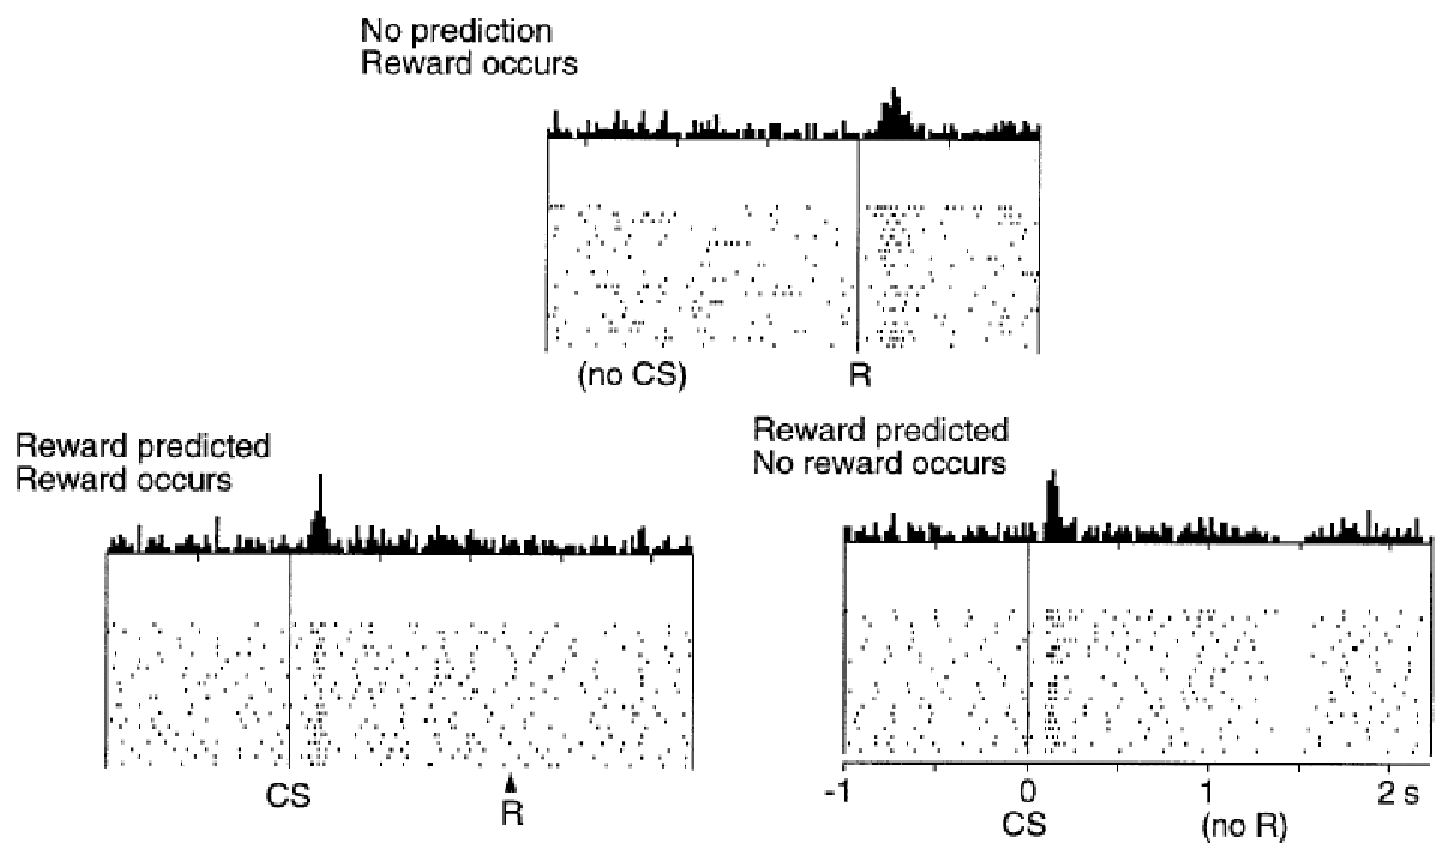
\includegraphics[width=15cm]{figures/schultz}
% \caption{Firing rates of midbrain dopamine neurons of the basal ganglia during classical conditioning (Adapted from Schultz et al., 1997)}
% \label{schultz}
%\end{figure}


\bigskip

\subsection{Computational Models of PFC}
The work presented in this chapter builds on an existing body of computational modeling work having strong ties to biology which includes a formal account of DA's affect on PFC functioning.  One of the primary insights of some recent models of PFC functioning is that the DA based TD learning mechanism might be used to learn, from experience, when to robustly maintain current representations in the PFC versus allowing updating to occur~\cite{BraverTS:2000:Control}.  As described earlier, it is helpful to think of the maintenance versus updating of PFC in terms of a gating mechanism.  When the gate is closed, the PFC representations are robustly maintained and protected from interference.  When the task contingencies change, the gate can be opened to allow for a more useful PFC goal or rule to be maintained to influence further processing. The key insight is that it might be possible to use the TD based error signal to learn \emph{covert} actions, such as when to open and when to shut the gate on PFC representations. By building computational models of PFC function, researchers have shown that this account is plausible~\cite{BraverTS:2000:Control,OReillyRC:2002:IDED}. In these models, a modeled PFC is included to actively maintain abstract task dimensions across the firing patterns of the modeled PFC units.  For instance, the PFC layer can encode, and actively maintain, a representation such as ``pay attention to the color of the stimuli''.  This maintained pattern of activity can then provide a ``top-down'' bias or up-modulation of pathways in posterior brain areas associated with the processing of stimulus color~\cite{CohenJD:1990:Stroop}.  The extra biasing provided by the PFC can be used to drive weaker, less automatic, behaviors (e.g. naming the color as opposed to reading the word in the Stroop task) when appropriate.  This activation based modulation is thought to be key to our ability to provide cognitive control over behavior~\cite{CohenJD:1992:Schizophrenia}.  The DA based adaptive gating mechanism can be used, within this context, as a way to signal to PFC when it is appropriate to strengthen the maintenance of the representation currently encoded (i.e. close the gate).  This occurs when a positive TD Error arises, signifying a positive change in expected future reward.  In other words, when the system is doing better than expected, close the gate on PFC representations so we are more likely to keep doing the same thing.  Conversely, when the network starts performing worse than expected, possibly due to task contingencies changing, this will result in a negative TD Error, signaling that the system is not performing as well as expected, and indicating that the system should adapt its behavior to perform more optimally.  The negative TD error can be used as a gating signal on the PFC representations, signaling the gate to open, allowing a new representation to replace the old, thereby allowing the network to flexibly adjust its control over behavior.

Along with providing a neural mechanism that can learn to appropriately and adaptively gate PFC representations, these models have also been successful in tying frontal disturbances, such as those found in schizophrenia, to deficits in cognitive control~\cite{CohenJD:1992:Schizophrenia} and cognitive flexibility~\cite{BraverTS:1999:Schizophrenia,OReillyRC:2002:IDED}.  A recent elaboration of this model, XT~\cite{RougierNP:2005:XT}, is the first neuroscientific model able to provide quantitative fits to a hallmark task of cognitive control, the Stroop task, and a widely used measure of cognitive flexibility, WCST, in both neurologically intact and frontally damaged people.  In the next chapter, XT has been adapted to investigate whether a dysfunctional DA based gating mechansim can capture the specific executive profile of people with autism in WCST and Stroop.  


%\subsection{The Problem with Overfitting}

%Cohen was the first researcher to report on a neural network model designed to explain patterns of behavior in people with ASD~\cite{CohenIL:1994:AutismLearning}.  Cohen's model rests on the notion that neural networks, when allowed to have too many units in a hidden layer, are likely to fall prey to the problem of ``overfitting'' the training data.  When training a neural network, one wishes to capture the true functional form (or at least the best possible approximation) of the task, as implicitly characterized by the training data.  By capturing the form of the function, the model is able to generalize to inputs that it has not been exposed to in the past.  When ``overfitting'' occurs, instead of capturing the true underlying functional form, the model essentially memorizes the specific training data items.  This results in precisely correct performance when the network experiences the training situations again, but poor performance on novel inputs.  In other words, overfitting results in poor generalization.  

%Cohen cites studies that have found that many areas of the brain, with a particular focus on the amygdala and hippocampus, exhibit an overall increase in the number of neurons in people with autism as compared to controls, Cohen argues that an analog between overfitting in neural networks and poor generalization, as seen in people with ASD, can be made.  Cohen conjectures that since the amygdala is implicated in emotional and social processing, too many neurons could result in a kind of ``overfitting'' of socially relevant stimuli, resulting in unrelated and unimportant features of a social situation being taken into account when learning appropriate social behavior.  The unrelated information will usually only hinder the ability to act appropriately in the extremely subtle and complex acts of social interactions, explaining the overall poor social abilities and lack of ability to generalize to new situations found in people with ASD.  A computational model is provided which demonstrates that, as the number of hidden layer units increase, the ability of the network to generalize to new inputs deteriorates.  Furthermore, it is argued that the savant-like abilities found in some people with autism can be explained as an overall increase in the number of neurons which are employed in the task.  For instance, Cohen suggests that if a person with autism has an extraordinary ability in a specific modality then, according to his theory, we should find an increased number of neurons in the network facilitating the learning of that modality (e.g., visual) and not in areas used for other modalities (e.g., haptic or auditory).

%Cohen's hypothesis of ``too many'' neurons resulting in a type of behavioral ``overfitting'' has some intuitive appeal, especially when analyzing how neural networks perform as a function of the number of processing units.  However, the model does not possess any solid fits to any specific quantitative behavioral data.  Instead it relies on a more abstract, verbally justified, account of how poor generalization arises in people with ASD.  Also, links to underlying neurobiological systems are of an almost anecdotal nature, casually noting that some postmortem studies have found an increased number of neurons in some areas of the brain in people with autism.

%\subsection{Inadequate Cortical Feature Maps}
%Gustafsson's modeling of inadequate cortical feature maps in autism follows in the footsteps of Cohen's attempt to explain good discrimination skills and poor generalization skills found in people with ASD~\cite{GustafssonL:1997:AutismMaps}.  In this endeavor, Gustafsson argues that overly narrow neural columns in people with autism are at the core of this pattern of behavior.  Cortex is believed to be organized in a columnar manner, with the neurons in each column possessing similar receptive field properties.  Neurons within a column in cortex tend to respond to the same aspects of a stimulus, resulting in a type of ``cortical feature map''.  If these neural columns are overly narrow, then, as Gustafsson writes, ``feature detection will only be possible if the set of features very closely corresponds to that which the neural column has become identified with, i.e., there must not be much variability in features'', and he follows, ``an individual with such an inadequate feature map must insist on precision or `sameness' ''.  This desire for ``sameness'' is a common behavioral feature found in people with ASD.  The thrust of the inadequate feature map hypothesis is that narrower neural columns in cortex will have narrower receptive field properties (responsive to a smaller than normal range of stimuli) and therefore exhibit good discrimination but poor generalization.

%The artificial neural network discussed in Gustafsson's 1997 article is based on networks developed by Kohonen~\cite{kohonen84selforg}, which include excitatory and inhibitory lateral feedback connections in a neighborhood-like structure.  This means that units within a certain distance of each other will contain mutually excitatory connections, while outside of this distance the connections to other units will be inhibitory~\cite{vod_der_MalsburgC:1973:SOM_Striate}.  This relationship causes a topological structure to develop in the models, with columnar-like groupings of units which respond in a similar manner to stimulus features.  An important property of these networks is that the Kohonen map learns its fundamental properties through extensive exposure to stimuli.  No set structure for stimulus representation is assumed to exist a priori.  This property allows for the possibility that inadequate feature maps will arise somewhat naturally during development, simply by manipulating a single parameter, namely increasing the level of lateral inhibition, in the model.  Gustafsson proceeds to provide a mathematical proof, based on previous findings~\cite{kohonen84selforg}, that as you increase the overall lateral inhibition, the columns in the Kohonen maps become narrower and respond to a smaller set of stimulus features.  In other words, they develop smaller receptive fields.

%Unlike the previous models, Gustafsson's model makes strong contact with underlying biological mechanisms.  However, considering the high comorbidity of seizures in the disorder it is unclear whether excessive lateral inhibition is justified~\cite{Casanova:2003:AutismMiniColumns}.  It is difficult to analyze the performance of the model, as no actual model simulation results were presented.  Therefore, the same critique of Cohen's work holds for Gustafsson's model: there is no evidence that the model will be able to provide a tight quantitative fit to actual behavioral data.   

%\subsection{Weak Central Coherence as Constraint Satisfaction}

%O'Loughlin and Thagard provide a computational modeling account of Frith's theory of weak central coherence~\cite{FrithU:1989:AutismWCC} by simulating coherence using a constraint satisfaction network~\cite{OLoughlinC:2000:Coherence}.  A constraint satisfaction problem can be roughly described as follows: Given a set of possible states of the world, of which some states may be less likely to coincide simultaneously with  others (e.g., it is not likely to be outside while it is raining, and not get wet), what set of states maximally satisfy all possible constraints?  A constraint satisfaction network embodies a constraint satisfaction problem where the different aspects of possible states of the world are specified as nodes in the network, and the constraints between these states are embodied by numeric weights on the connections between these nodes.  For an exclusivity constraint between two different states (representing the concept that the two states are not likely to occur together, e.g., eating and being asleep at the same time), a negative weight value is used, and for a co-occurrence constraint (representing when the two states are likely to occur together, e.g., being thirsty and drinking water) a positive weight value is used.  ``Normal'' coherence is taken to be the network functioning in the standard manner, maximally choosing the states which satisfy the most constraints.  WCC is simulated as pushing the network to settle upon a sub-optimal set of states, which do not maximally satisfy all of the constraints. 

%To make this more clear, it is helpful to consider the simulation provided by O'Loughlin and Thagard using the Sally-Anne task~\cite{Baron-Cohen:1985:AutismTOM}.  To simulate this task, the nodes of the network are coded to represent possible states in the task such as ``Sally puts marble in basket'' and ``Anne transfers marble to box while Sally is away'', with positive connections (positive constraint) between the states and negative connections (negative constraints) between nodes such as ``Sally looks in basket'' and ''Sally looks in box''.  The different states and constraints between them represent a kind of ``knowledge network'' of the Sally-Anne task.  If the constraints are set up properly, the network will settle on the correct hypothesis, that ``Sally looks in basket''.  

%In order to simulate WCC as seen in children with autism, the negative constraints (connections) were increased, making the inhibitory connections stronger than the excitatory connections.  This manipulation results in the network settling prematurely and most likely in a state that did not satisfy all of the original constraints in the network.  In the simulation of the Sally-Anne task, the solution resulting in the incorrect choice of ``Sally looks in box'' is essentially ``shorter'' and simpler than the correct, but unfortunately more causally complex, choice ``Sally looks in basket''.  This allows the increased inhibition to result in the network guessing incorrectly, ``Sally looks in box'', since when the network has finished the settling process, it will satisfy the most modified constraints in the constraint satisfaction network.

%The modeling approach used is extremely abstract in nature, with all of the knowledge of how the problem is to be solved pre-specified within the structure of the network (i.e., the nodes and the constraints between them).  It is unclear whether the mechanism employed to simulate performance of people with autism on the Sally-Anne task, namely increased inhibition in the network, can be biologically supported, considering, once again, the high comorbidity of seizures in the disorder~\cite{Casanova:2003:AutismMiniColumns} as well as lack of any other justification from the authors.  While the model is used to capture qualitative behavioral performance on the Sally-Anne task (as well as an example of a homograph task using the same approach), it is unclear how the model would fare at capturing quantitative behavioral data on these tasks.


%\subsection{Hyperspecificity}
%McClelland takes a slightly different approach to the same issues of poor generalization and stimulus overselectivity (or hyperspecificity) addressed by the models previously mentioned~\cite{McClellandJL:2000:Autism}.  Instead of providing a model, or even a description of a model, McClelland provides a general description of some of the properties of neural networks which could give rise to hyperspecificity at the cost of the ability to generalize.  Conjunctive codes in neural networks are representations that consist of components that, instead of responding to individual features of input (e.g., either ``red'' or ``square''), only respond to conjunctions of the input features (e.g., ``red square'').  As the number of conjuncted features required to activate a processing unit increases, the network's representation of the current situation becomes more specific (e.g., only responding to small green circles with radial lines, etc.).  Conjunctive representations are useful when the stimulus is actually a conjunction of features (e.g., a chair is a conjunction of many smaller components such as the seat, legs, back, etc.), however, this coding scheme can hinder generalization, since each unit only responds to a specific conjunction of features.  McClelland introduces the possibility that children with autism posses overly conjunctive representations of the environment.  This could account for hyperspecificity found in people with ASD.  McClelland provides an anecdotal story of a child with autism who refuses to use the restroom at a friends house because it is unfamiliar.  In other words, it is not the specific bathroom with which he is familiar.  If we think of the bathroom which the child with autism uses at his home, it may posses items such as green walls, a toilet, tile on the floor, etc., none of which are present in the friends home, with the likely exception of the toilet.  Perhaps, McClelland argues, the child represents the toilet with an overly conjunctive representation that includes other contextual items such as the color of the walls, the tile on the floor, etc.  

%Perhaps the largest problem with McClelland's modeling theory of hyperspecificity in autism is that no computational model ---not even a precise \emph{description} of a model--- is provided.  Many details would need to be specified before such a general verbal description could be brought in contact with quantitative behavioral data.  Also, the theory does not address what neurobiological differences in people with autism might give rise the overly conjunctive code argued to provide a possible account of hyperspecificity in ASD\footnote{McClelland is no longer a proponent of the overly-conjunctive hypothesis described here (Personal Communication, 2007).}.

%\subsection{iSTART}
%Grossberg \& Seidman (2006)~\nocite{RefWorks:146} provide a recent, ambitious, and complex computational model seeking to explain behavior in people with autism to date, known as iSTART (Imbalanced Spectraly Timed Adapative Resonance Theory).  The iSTART model of autistic performance stands on the shoulders of three previous modeling frameworks, ART --- ``Adaptive Resonance Theory'', CogEM --- ``Cognitive - Emotional - Motor'', and the ``Spectral Timing'' model.  ART proposes how the brain learns to categorize objects and events.  According to ART, when an object is experienced in the environment, perceptually driven bottom-up representations are compared with previously learned top-down expectations. If there is sufficient overlap or similarity between top-down and bottom-up representations, then a ``recognition process'' is instantiated.  However, if there is not sufficient similarity, then the object is determined to be novel, and a different process is instantiated to add the object as a new category.  The amount of similarity that is required to determine whether an object is novel or not is determined by a single parameter termed ``vigilance''.  It is proposed that people with autism are hyper-vigilant, resulting in overly specific category structures.  The hyper-specific category structures are argued to be at the root of the overly specific kinds of processing demonstrated by people with autism and traditionally accounted for by theories such as weak central coherence.  

%It is unclear how the vigilance manipulation would be able to account for the overselective behavior seen in people with autism.  Rather, the prediction of the model seems to be that all aspects of the objects are processed, just in a highly componential manner.  This would result in overly specific representations that do not promote generalization, but it does not provide any insight for why certain features might dominate processing.  

%A second portion of the iSTART framework, CogEM, extends the ART framework to %account for cognitive-emotional associations.  Within this framework, %``under-aroused'' emotional circuits are posited to be a problem for some people with autism.  The functional implications of a CogEM emotional circuit being under-aroused are two-fold. First, the threshold for activation of an emotion is higher than normal.  This is argued to be an explanation for the lack of emotional responstivity in people with ASD.  The second consequence of under-aroused emotional circuits in CogEM are heightened reactions to stimuli after this high emotional threshold has been reached.  Heightened reactions, according to the authors, are synonymous with and an explanation for the emotional outbursts seen in people with autism. 

%The final portion of iSTART, Spectral Timing, is used to explain how the brain learns to adaptively time responses in order to maximize the acquisition of rewards in the environment.  For instance, when an animal is conditioned to expect reward two seconds after a lever press, what mechanism prevents learning the association of non-reward during that two second interval?  Furthermore, how can the animal learn that once this two second interval has passed its earlier expectation of reward was false?  Clearly some timing mechanism is necessary in order to accomplish learning in situations involving temporally delayed reward.  Grossberg et al. propose that such a timing mechanism may be perturbed in people with autism.  Without an adequate ability to properly learn in temporally contingent situations, such as nearly all social situations, people with autism will obviously struggle. 

%The iSTART model is argued to be able to account for many aspects of behavior in people with autism through a ``system-wide vicious circle of environmentally mediated feed back'' causing and maintaining problems across the three different models which comprise iSTART.  While ambitious in its breadth, the iSTART model of autism never accounts for behavior in people with autism through more than a purely verbal argument and description of how the model should function.  No quantitative fits to data are shown, nor give any qualitative model results provided to help demonstrate the model predictions.  Complex computational models, such as iSTART, can be very difficult to evaluate in a purely analytical manner.  Often, surprising and unanticipated results may occur.  Actual modeling results comparing model performance to behavioral data collected from people with autism would be extremely useful.  For instance,  simulation results can be helpful in answering questions concerning whether iSTART is capable of accounting for important behavioral results which appear problematic for the framework, such as overselective behavior.  

%\subsection{Issues with Previous Models of Autism}
%%%Most of the existing models of autism reviewed above are fairly abstract in nature, making little contact with specific neurobiological considerations~\cite{CohenIL:1994:AutismLearning,McClellandJL:2000:Autism,OLoughlinC:2000:Coherence}.  Even those models of autism which have incorporated biology into their framework have thus far only matched qualitative patterns of behavior in people with ASD, not attempting to account for any quantitative behavioral data~\cite{GustafssonL:1997:AutismMaps,RefWorks:146}.  Models more tightly coupled with observed functional properties of neurobiological systems and constrained by actual behavioral data will be able to more precisely inform theories of ASD. 

%\subsection{Dopamine \& Temporal Difference Learning}
%Our account of the role of dopamine in autistic behavior builds on recent findings concerning the midbrain dopamine system and its relationship to the prefrontal cortex. Hidden within the firing rates of midbrain DA neurons lie clues to how the intelligent updating of PFC might be implemented in the neural hardware of the brain.  Analyzing the response profile of DA neurons in the basal ganglia of monkeys, Schultz et al. (1997)~\nocite{schultz97td} have demonstrated that DA cells appear to encode a prediction error in the amount of future reward to be given to the monkey.  In other words, these cells seem to encode a \emph{change in expected future reward}.  Figure~\ref{schultz} shows results from a population of midbrain DA cells during one of Schultz's experiments.  The top panel represents the situation in which the monkey is not expecting reward, but then receives reward (e.g., a sip of juice).  Notice that the DA cells fire upon receiving the reward (signified by ``R'' on the graph), encoding a positive change in what the monkey was expecting.  In the bottom left panel, the monkey has now been conditioned to associate a flash of light with the delivery of the juice, after a short delay.  In other words, the monkey now knows that the flash of light predicts future reward.  When the flash of light is seen (represented as ``CS'', for ``conditioned stimulus'', in the graph), the DA cells fire.  This can be explained as the monkey expecting future reward once the light comes on, signaling that juice is expected to be coming soon: a positive change in expected future reward.  However, when the reward is delivered (``R'') the cells to do not fire, since the monkey was already expecting reward.  When the juice is delivered there is no change in expected future reward, in this case, and, therefore, no increase in the rate of DA firing.  In the panel located at the bottom right, the DA cells again fire for the flash of light (``CS'', conditioned stimulus) , but this time the experimenters \emph{withhold the juice} at the time when the monkey is expecting the juice to be delivered.  The monkey is \emph{expecting} reward, but no reward is delivered. Thus, at the time that juice is expected, there is a negative going change in expected future reward.  Notice that the firing rates of the DA cells around the expected delivery time of reward (``R'') actually dip below their baseline firing rate and, indeed, appear to encode this negative change in expected future reward.

%This is very interesting because change in expected future reward is also the key variable in a very powerful reinforcement learning algorithm known as Temporal Difference (TD) learning.  In TD learning, the change in expected future reward, the same value the DA cells appear to be encoding, is know as the TD Error.  Across two consecutive time steps the TD Error is given by: 
%\begin{equation}\delta(t) = r(t) + \gamma V(t+1) - V(t)\end{equation}

%Where $r(t)$ is a continuous reward value that is delivered at each time step based on system performance (e.g., $r(t) = 1$ for correct performance and $r(t)=0$ on time steps when no reward is presented), $V(t)$ and $V(t+1)$ are the expected future rewards at times $t$ and $t+1$ respectively, \begin{math}\delta(t)\end{math} is the change in expected future reward, or TD Error, and \begin{math}\gamma\end{math} is a constant discounting factor, where \begin{math}0 < \gamma \leq 1\end{math}.  Adjusting \begin{math}\gamma\end{math} changes the amount by which temporally distant rewards are discounted as compared to rewards that can be attained in the temporally near future. 

%Linking machine learning and neurobiology, this connection has led researchers to formalize the role of midbrain DA neurons in the brain's learning mechanisms~\cite{BartoAG:1994:TDLearning,MontaguePR:1996:Dopamine}, equating the firing rate of the DA cells with the amount of change in expected future reward, or TD Error.  Neurally plausible implementations of TD learning have been implemented and have been used to model the learning of motor sequences in the striatum~\cite{MontaguePR:1996:Dopamine}, driven by the reward-prediction DA signal.


%\begin{figure}
% 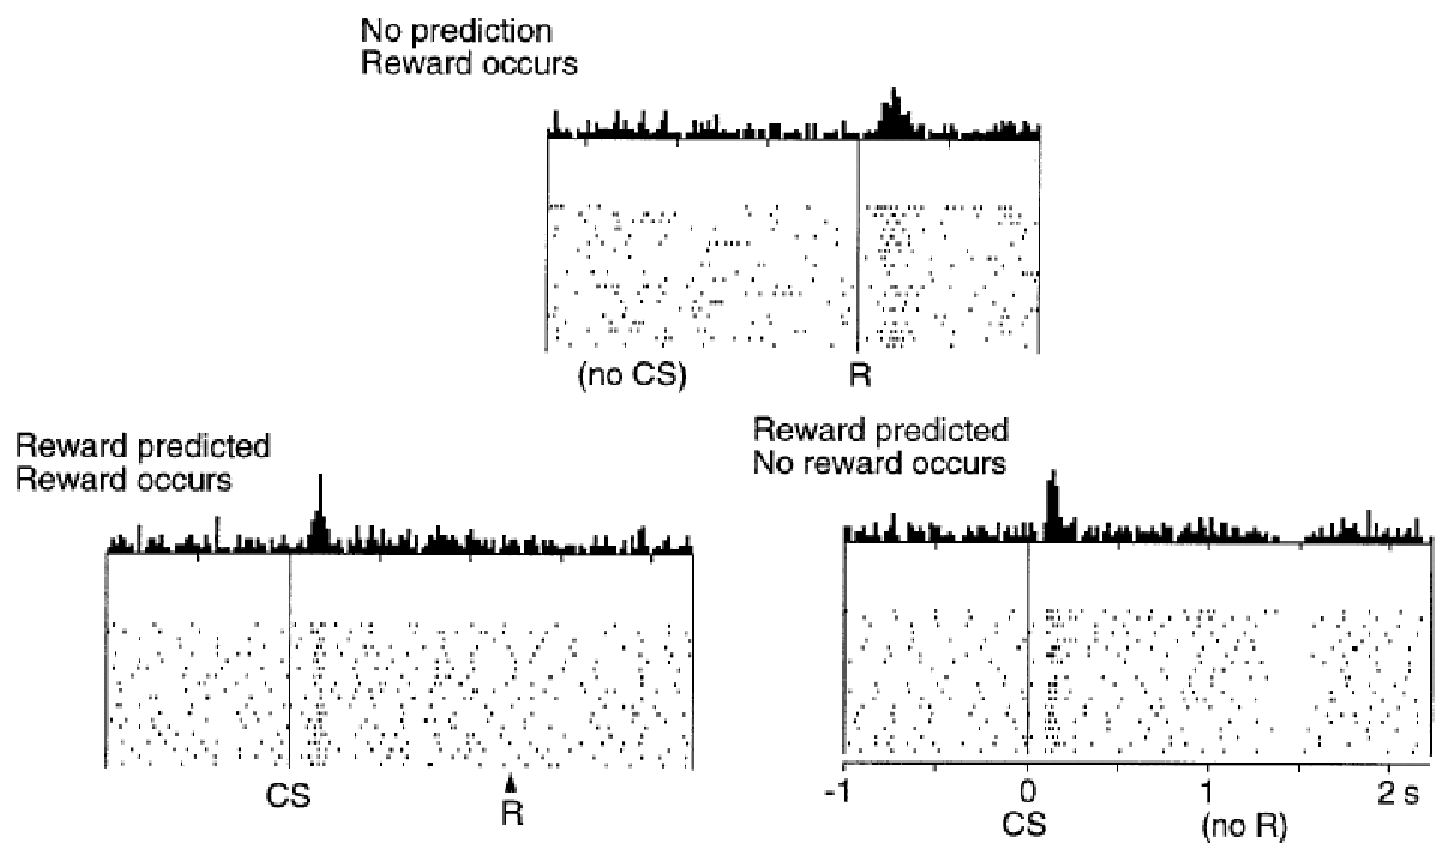
\includegraphics[width=15cm]{figures/schultz}
% \caption{Firing rates of midbrain dopamine neurons of the basal ganglia during classical conditioning (Adapted from Schultz et al., 1997)}
% \label{schultz}
%\end{figure}


%\bigskip

%\subsection{Computational Models of PFC}
%My current work builds on an existing body of computational modeling work having strong ties to biology which includes a formal account of DA's affect on PFC functioning.  The effect of DA is formalized by equating the firing rate of midbrain DA neurons to the key variable, the TD Error, of the powerful TD learning algorithm.  Using this connection between biology and machine learning, researchers have been able to provide models of how motor systems can learn sequences of overt actions leading to reward.  One of the primary insights of some recent models of PFC functioning is that the DA based TD learning mechanism might be used to learn, from experience, when to robustly maintain current representations in the PFC versus allowing updating to occur~\cite{BraverTS:2000:Control}.  As described earlier, it is helpful to think of the maintenance versus updating of PFC in terms of a gating mechanism.  When the gate is closed, the PFC representations are robustly maintained and protected from interference.  When the task contingencies change, the gate can be opened to allow for a more useful PFC goal or rule to be maintained to influence further processing.  The key insight is that, if TD can be used to learn sequences of \emph{overt} actions, it might be possible to use this same error signal to learn \emph{covert} actions, such as when to open and when to shut the gate on PFC representations.  By building computational models of PFC function, researchers have shown that this account is plausible~\cite{BraverTS:2000:Control,OReillyRC:2002:IDED}.  A layer of processing units representing  the PFC is included in these models, and this layer is used to actively maintain abstract task dimensions across the firing patterns of the units.  For instance, the PFC layer can encode, and actively maintain, a representation such as ``pay attention to the color of the stimuli''.  This maintained pattern of activity can then provide a ``top-down'' bias or up-modulation of pathways in posterior brain areas associated with the processing of stimulus color~\cite{CohenJD:1990:Stroop}.  The extra biasing provided by the PFC can be used to drive weaker, less automatic, behaviors (e.g. naming the color as opposed to reading the word in the Stroop task) when appropriate.  This activation based modulation is thought to be key to our ability to provide cognitive control over behavior~\cite{CohenJD:1992:Schizophrenia}.  The DA based adaptive gating mechanism can be used, within this context, as a way to signal to PFC when it is appropriate to strengthen the maintenance of the representation currently encoded (i.e. close the gate).  This occurs when a positive TD Error arises, signifying a positive change in expected future reward.  In other words, when the system is doing better than expected, close the gate on PFC representations so we are more likely to keep doing the same thing.  Conversely, when the network starts performing worse than expected, possibly due to task contingencies changing, this will result in a negative TD Error, signaling that the system is not performing as well as expected, and indicating that the system should adapt its behavior to perform more optimally.  The negative TD error can be used as a gating signal on the PFC representations, signaling the gate to open, allowing a new representation to replace the old, thereby allowing the network to flexibly adjust its control over behavior.

%Along with providing a neural mechanism that can learn to appropriately and adaptively gate PFC representations, these models have also been successful in tying frontal disturbances, such as those found in schizophrenia, to deficits in cognitive control~\cite{CohenJD:1992:Schizophrenia} and cognitive flexibility~\cite{BraverTS:1999:Schizophrenia,OReillyRC:2002:IDED}.  A recent elaboration of this model, XT~\cite{RougierNP:2005:XT}, is the first neuroscientific model able to provide quantitative fits to a hallmark task of cognitive control, the Stroop task, and a widely used measure of cognitive flexibility, WCST, in both neurologically intact and frontally damaged people.  In the next chapter, XT has been adapted to investigate whether a dysfunctional DA based gating mechansim can capture the specific executive profile of people with autism in WCST and Stroop.  
